\documentclass[letterpaper,11pt]{article}
\usepackage{epsfig,latexsym,amsmath,amssymb,epic,eepic,psfrag,subfigure,float,euscript,array}
\usepackage[latin1]{inputenc}
\usepackage{standalone}
\usepackage{tikz,pgf,pgfplots}
\usepackage[margin=2.5cm]{geometry}
\usepackage[amssymb]{SIunits}

\newenvironment{exercise}[1][Uppgift]{\begin{trivlist} \item[\hskip
    \labelsep {\stepcounter{exerctr}\bfseries #1
      \arabic{exerctr}}]}{\end{trivlist}\vspace{10mm}}

\newcounter{exerctr}
\newcounter{abcctr}[exerctr]

\newcommand{\abc}{\noindent\vspace{1mm}\\ {\bf
    \stepcounter{abcctr}(\alph{abcctr})\ }}
\newcommand{\bbm}{\begin{bmatrix}}
\newcommand{\ebm}{\end{bmatrix}}
\newcommand{\point}[1]{\hfill {\bf (#1p)}\\ \vspace{-5mm}}
\newcommand{\ctrb}{\EuScript{S}}
\newcommand{\Lap}{\mathcal{L}}
\newcommand{\obsv}{\EuScript{O}}
\newcommand{\realdel}[1]{\text{Re}\left\{#1\right\}}
\newcommand{\imagdel}{\text{Im}}
\newcommand{\bC}{\mathbb{C}}
\newcommand{\bR}{\mathbb{R}}
\newcommand{\bmpv}{\begin{minipage}[t]}
\newcommand{\bmps}{\begin{minipage}[t]{45mm}}
\newcommand{\bmpm}{\begin{minipage}[t]{90mm}}
\newcommand{\bmpl}{\begin{minipage}[t]{\textwidth}}
\newcommand{\emp}{\end{minipage}}
\newcommand*{\zethree}{\big(z - \mexp{-3h}\big)}
\newcommand*{\mexp}[1]{\ensuremath{\mathrm{e}^{#1}}}

\newcommand*\circled[1]{\tikz[baseline=(char.base)]{
            \node[shape=circle,draw,inner sep=2pt] (char) {#1};}}

\addtolength{\topmargin}{-1cm}
\textheight 23.5cm
%\oddsidemargin 0.61cm
%\evensidemargin 0.61cm


\title{Computerized control partial exam 2 (15\%)}
\author{Kjartan Halvorsen}

\begin{document}

\maketitle


\begin{description}
\item[Time] 2017-10-24 17:35 - 19:00
\item[Place] 4209
\item[Permitted aids] The single colored page with your own notes, table of Laplace transforms, calculator
\end{description}

All answers should be readable and well motivated (if nothing else is written). Solutions/motivations should be written on the provided spaces in this exam. Use the last page if more space is needed.

\begin{center}
{\Large Good luck!} \\
\end{center}

\noindent
\fbox{
\bmpl
{\bf Matricula and name:}\\
\vspace*{30mm}
\emp}

\subsubsection*{Active mass damper system for highrise buildings}
%----------------------
% AMD
%----------------------
\noindent
\begin{minipage}{0.6\linewidth}
Many skyscrapers in windy and earthquake exposed regions around the world are built with damping devices to reduce vibrations and displacements from disturbances. The most common device is the passive \emph{tuned mass damper} as in the building Taipei 101 in Taipei, Taiwan, seen to the right. The idea is to connect a large mass to the building using springs and dampers. The mass of the damper, the spring stiffness and the damping coefficients are chosen in order to reduce the resonance of the building. Some damper systems also include active elements that may produce a force between the damping mass and the building. Figure \ref{fig:amd} shows a simple one-dimensional model of such a system.
\end{minipage}
\begin{minipage}{0.4\linewidth}
\begin{center}
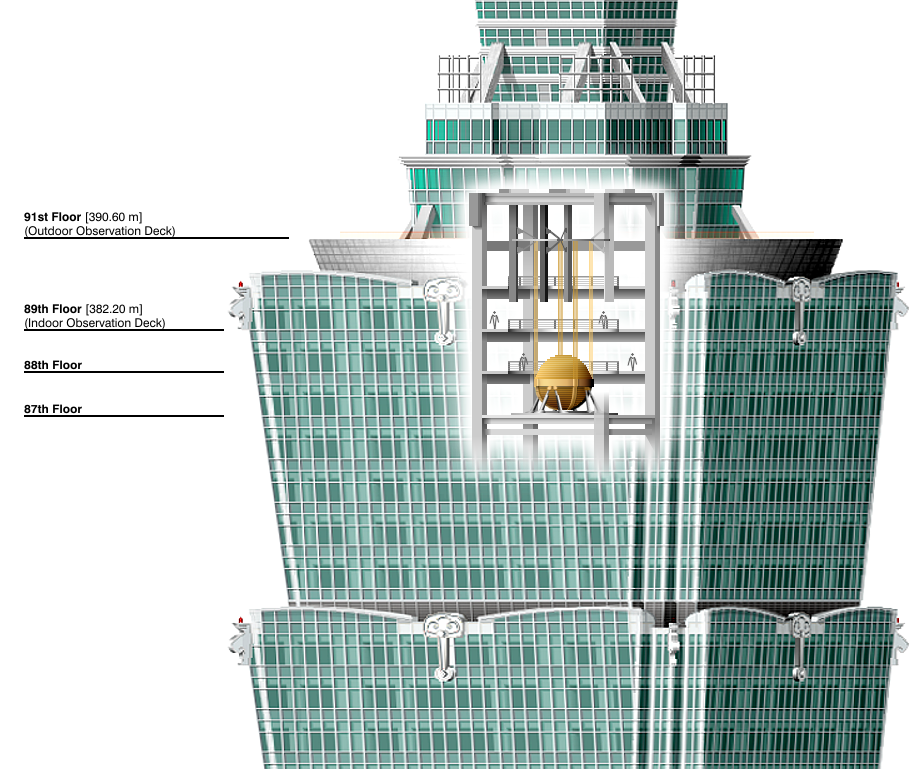
\includegraphics[width=\linewidth]{taipei-101.png}
\end{center}
\end{minipage}
\clearpage

\begin{figure}
\begin{center}
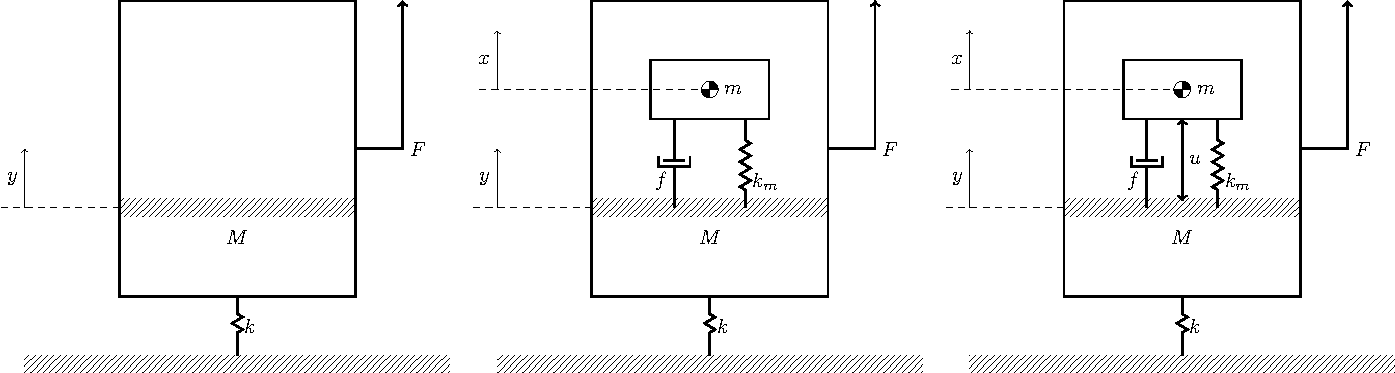
\includegraphics[width=\linewidth]{active-mass-damper-system-vertical}
\caption{One-dimensional model of mass damper system for buildings. The view is looking down at the building from straight above. In this simplified model the connection between the building and the ground is elastic with no damper. The left model shows a model of the building only, with no damping system. The middle model is a passive damper system, and the right one is an active damper system where actuators generate a force $u$ between the building and the damper mass. The force $F(t)$ is an external horizontal force due to wind or earthquake. The variable $x(t)$ is the displacement of the damper mass and $y(t)$ is the displacement of the building.}
\label{fig:amd}
\end{center}
\end{figure}
The undamped model of the building, the left-most model in figure \ref{fig:amd}, is clearly a harmonic oscillator with natural frequency \(\omega_n = \sqrt{\frac{k}{M}}\). With the tuned damper system (middle model), energy is dissipated by the damper pistons, which makes the response of the system more damped. The active system to the right gives further possibilities to attenuate the disturbance $F(t)$ through feedback from $y(t)$, but also through feedforward from measured disturbance $F(t)$, for instance from  accelerometers in the base of the building and wind speed sensors on the roof. 

\subsection*{Problem 1}
%----------------------
% RST design for the AMD
%----------------------

With some particular values of the masses $m$ and $M$, the spring constants $k$ and $k_m$ and damping coefficient $f$,  the following pulse-transfer function from the input $u$ to the output $y$ for the model with active damping (the right-most model in figure \ref{fig:amd}) is obtained
\begin{equation}
  H(z) = \frac{B(z)}{A(z)} = \frac{0.02 z^3 - 0.021 z^2 - 0.017 z + 0.018}{z^4 - 3.81 z^3 + 5.50 z^2 - 3.55 z+ 0.870}
\end{equation}
In order to improve the attenuation of the  disturbance $F(k)$, feedback control as in figure \ref{fig:dt} is considered. 
\begin{figure}[h]
\begin{center}
     \begin{tikzpicture}[scale = 0.8, node distance=25mm, block/.style={rectangle, draw, minimum width=15mm}, sumnode/.style={circle, draw, inner sep=2pt}]
     
     \node[coordinate] (refinput) {};
     \node[sumnode, right of=refinput, node distance=20mm] (sumerr) {\tiny $\sum$};
     \node[block, right of=sumerr] (controller) {$F(z) = \frac{S(z)}{R(z)}$};
     %\node[above of=controller, node distance=6mm] {controller};
     \node[block, right of=controller, node distance=35mm] (plant) {$H(z)$};
     \node[sumnode, right of=plant, node distance=24mm] (sum) {\tiny $\sum$};
     \node[block, below of=plant, node distance=14mm] (AA) {$z^{-2}$};
     %\node[above of=tank, node distance=6mm] {motor};
     \node[coordinate, right of=sum, node distance=20mm] (output) {};
     \node[block, above of=sum, node distance=14mm] (Gf) {$H_F(z)$};
     \node[coordinate, above of=Gf, node distance=10mm] (disturbance) {};

     \draw[->] (refinput) -- node[above, pos=0.1] {$y_{ref}=0$} (sumerr);
     \draw[->] (sumerr) -- node[above] {$e(k)$} (controller);
     \draw[->] (controller) -- node[above] {$u(k)$} (plant);
     \draw[->] (plant) -- (sum);
     \draw[->] (sum) -- node [coordinate] (measure)  {} node [above, near end] {$y(k)$} (output);
     \draw[->] (disturbance) -- node[right, pos=0.1] {$F(k)$} (Gf);
     \draw[->] (Gf) -- node[right, pos=0.1] {} (sum);
     \draw[->] (measure) |- (AA) -| node[right, pos=0.95] {$-$} (sumerr);
     \end{tikzpicture}
     \caption{Feedback control design in discrete time.}
     \label{fig:dt}
   \end{center}
 \end{figure}


\subsubsection*{(a)}
Determine the closed-loop pulse-transfer function from the disturbance $F(k)$ to the displacement $y(k)$ of the building.

\noindent
\fbox{
\bmpl
{\bf Calculations:}\\
\vspace*{60mm}
\emp}

\subsubsection*{(b)}
There is a pulse-transfer function $z^{-2}$ in the feedback path. What could this represent?

\noindent
\fbox{
\bmpl
{\bf Answer:}\\
\vspace*{15mm}
\emp}

\subsubsection*{(c)}
Determine the degree of the polynomials $R(z)$ and $S(z)$ of the controller $F(z) = \frac{S(z)}{R(z)}$ so that all the controller parameters can be determined from the Diophantine equation for the closed-loop system.

\noindent
\fbox{
\bmpl
{\bf Calculations:}\\
\vspace*{90mm}
\emp}


\subsubsection*{(d)}
When setting up the Diophantine equation, the desired characteristic polynomial $A_{cl}(z)$ of the closed-loop system goes on the right-hand side of the equation. The plant $H(z)$ has poles as shown in the pole-zero map below. \textbf{Mark} in the figure two desired closed-loop poles that you think are reasonable (we would of course need to specify more than two desired poles, though). \textbf{Motivate} your suggestion. Hint: Don't forget about practical limitations.

\begin{center}
  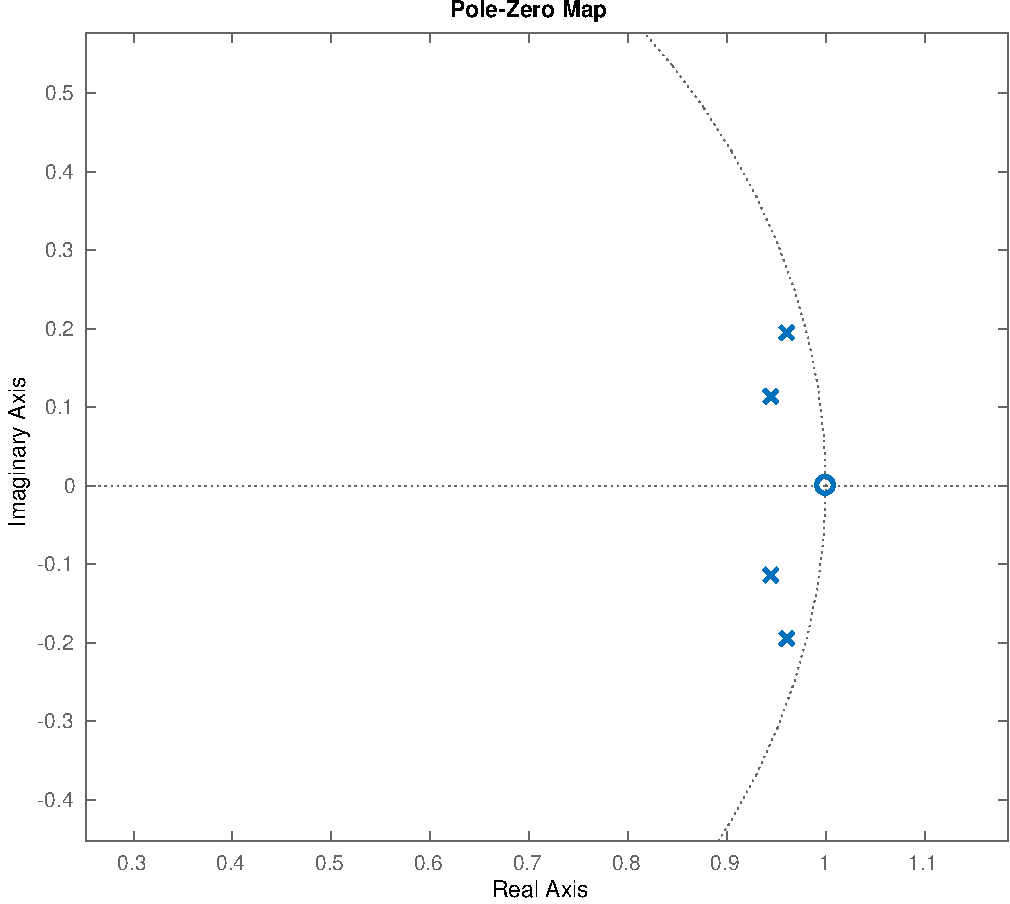
\includegraphics[width=0.6\linewidth]{amd_pzmap-crop}
\end{center}

\noindent
\fbox{
\bmpl
{\bf Motivation:}\\
\vspace*{50mm}
\emp}

%\clearpage
\subsection*{Problem 2}
Instead of the discrete-time design in Problem 1, consider a controller designed in the continuous time domain based on a continuous-time model $G(s)$ of the system with active mass damping. See figure \ref{fig:ct}. 
\begin{figure}[h]
\begin{center}
     \begin{tikzpicture}[scale = 0.8, node distance=25mm, block/.style={rectangle, draw, minimum width=15mm}, sumnode/.style={circle, draw, inner sep=2pt}]
     
     \node[coordinate] (refinput) {};
     \node[sumnode, right of=refinput, node distance=20mm] (sumerr) {\tiny $\sum$};
     \node[block, right of=sumerr] (controller) {$F(s)$};
     %\node[above of=controller, node distance=6mm] {controller};
     \node[block, right of=controller, node distance=35mm] (plant) {$G(s)$};
     \node[sumnode, right of=plant, node distance=24mm] (sum) {\tiny $\sum$};
     %\node[above of=tank, node distance=6mm] {motor};
     \node[coordinate, right of=sum, node distance=20mm] (output) {};
     \node[block, above of=sum, node distance=14mm] (Gf) {$G_F(s)$};
     \node[coordinate, above of=Gf, node distance=10mm] (disturbance) {};

     \draw[->] (refinput) -- node[above, pos=0.1] {$y_{ref}(t)=0$} (sumerr);
     \draw[->] (sumerr) -- node[above] {$e(t)$} (controller);
     \draw[->] (controller) -- node[above] {$u(t)$} (plant);
     \draw[->] (plant) -- (sum);
     \draw[->] (sum) -- node [coordinate] (measure)  {} node [above, near end] {$y(t)$} (output);
     \node[sumnode, below of=measure, node distance=14mm] (sumnoise) {\tiny $\sum$};
     \draw[->] (disturbance) -- node[right, pos=0.1] {$F(t)$} (Gf);
     \draw[->] (Gf) -- node[right, pos=0.1] {} (sum);
     \draw[->] (measure) -- (sumnoise);
     \draw[->] (sumnoise) -| node[right, pos=0.9] {$-$} (sumerr);
     \draw[->] (sumnoise) ++ (12mm, 0) -- node[above, near start] {$n(t)$} (sumnoise);
     \end{tikzpicture}
     \caption{Feedback control design in continuous time.}
     \label{fig:ct}
   \end{center}
 \end{figure}
 

\subsubsection*{(a)}
The controller $F(s) = \frac{0.5s + 0.15}{s+1}$ has been found to give reasonable performance. \textbf{Sample} the controller $F(s)$ for arbitrary sampling period $h$ using Tustin's approximation, and determine the zero and the pole of the discrete-time controller. 

\noindent
\fbox{
\bmpl
{\bf Calculations:}\\
\vspace*{100mm}
\emp}



\subsubsection*{(b)}
The figure below shows magnitude part of the Bode diagram of the closed-loop system from the measurement noise $n(t)$ to the output $y(t)$.  
\begin{center}
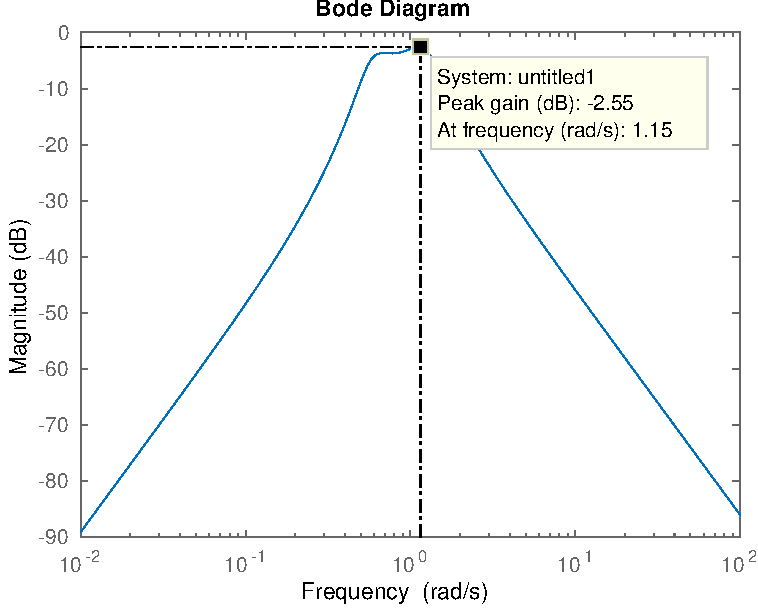
\includegraphics[width=0.5\linewidth]{amd_bode_Gc_magn-crop}
\end{center}


\textbf{Explain}, based on the Bode diagram above and/or from an intuitive understanding of how the active damper system works, why a constant measurement noise \(n(t)=n_0\) (a sensor bias) will not give a steady-state displacement $y(t)$ of the building.

\noindent
\fbox{
\bmpl
{\bf Explanation:}\\
\vspace*{60mm}
\emp}

\subsubsection*{(c)}
The computer-controlled system based on the design in figure \ref{fig:ct} requires sampling of the measured signal \(y_m(t) = y(t) + n(t)\). The chosen sampling frequency is \(\omega_s = \unit{378}{\radian\per\second}\). Unfortunately, the control engineers have made the error of completely ignoring a significant sinusoidal measurement noise $n(t)$ with frequency \unit{60}{\hertz}, originating from the electrical grid. What is the \textbf{alias frequency} in the frequency band (0, \(\omega_N\)) of this sinusoidal signal? What is the \textbf{consequence} of ignoring this measurement noise? How should the engineers \textbf{modify} their control system?     

\noindent
\fbox{
\bmpl
{\bf Calculations and answers:}\\
\vspace*{110mm}
\emp}
\cleardoublepage

\noindent
{\bf If necessary,} you can continue your solutions on this sheet. Mark clearly which problem the solution corresponds to.

%\end{document}

\section*{Solutions}
\subsection*{Problem 1}
\subsubsection*{(a)}
The loop gain is \(H_o(z) = F(z)H(z)z^{-2}\). Using Mason's rule we get for the closed-loop transfer function from the disturbance $F$ to to output $y$
\[ H_{cf} = \frac{H_F(z)}{1 + H_o(z)} = \frac{H_F(z)}{1 + \frac{S(z)}{R(z)}\frac{B(z)}{A(z)}z^{-2}}
          = \frac{H_F(z)A(z)R(z)z^2}{A(z)R(z)z^2 + B(z)S(z)}.\]

\subsubsection*{(b)}
A pulse-transfer function \(z^{-2}\) is simply a delay of two sampling periods. Most likely, this is included in the model to represent the delay in the feedback path due to an antialiasing filter.

\subsubsection*{(c)}
The Diophantine equation for this system is 
\[ A(z)R(z)z^2 + B(z)S(z) = A_{cl}(z),\]
with degree given by \( \deg A + \deg R + 2\). We get this many equations in the unknown controller parameters. The controller is given by 
\[F(z) = \frac{S(z)}{R(z)} = \frac{s_0z^n + s_1z^{n-1} + \cdots + s_n}{z^n + r_1z^{n-1} + \cdots + r_n},\]
where we have used to common choice of letting the numerator and denominator of the controller have the same degree. The controlle has \(2n + 1 = 2\deg R + 1\) unknown parameters. In order to determine all of this from the Diophantine equation, we must have
\[ \deg A + \deg R + 2 = 2\deg R + 1 \quad \Rightarrow \quad \deg R = \deg A + 1 = 5.\]

\subsubsection*{(d)}
Motivation for reasonable choice of closed-loop poles: The plant is clearly oscillatory due to the (fastest) pair of poles close to the unit circle, and with a certain frequency given by the angle to the real axis of the poles. To make the closed-loop system  behave very different from the natural behaviour of the plant requires large input signals. In practice the size of the input signal is restricted by the actuators. There are physical limitations provided by the comparatively small damping mass (compared to the building) and the possible forces that can be exerted between the damping mass and the building. It is therefore reasonable to desire poles that are somewhat more damped, and with about the same natural frequency as the plant poles. For instance as the red poles in the figure below 
\begin{center}
  \begin{tikzpicture}
    \node {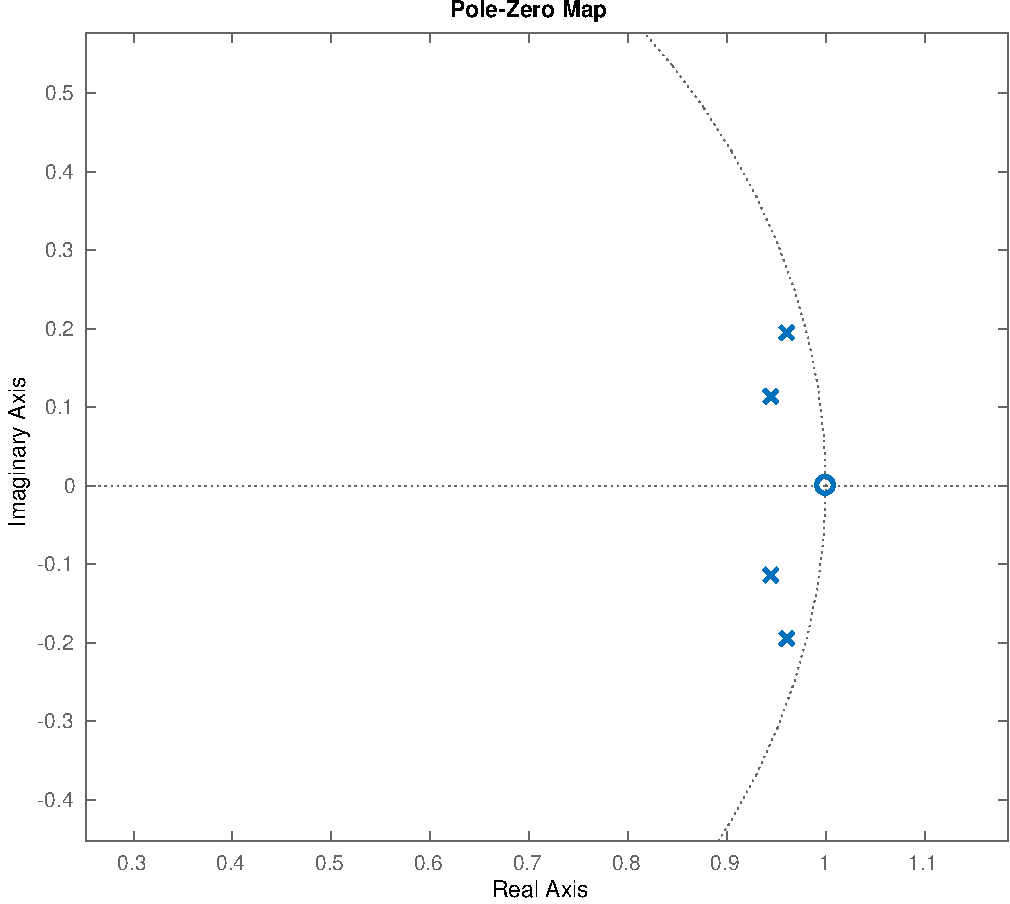
\includegraphics[width=0.6\linewidth]{amd_pzmap-crop}};
    \node[color=red!80] at (2.6cm, 1.03cm) {\Large $\times$};
    \node[color=red!80] at (2.6cm, -1.7cm) {\Large $\times$};
  \end{tikzpicture}
\end{center}

\subsection*{Problem 2}

\subsubsection*{(a)}

Discretizing the controller using Tustin's approximation
\begin{equation*}
  \begin{split}
    F_d(z) &= F(s)|_{s=\frac{2(z-1)}{h(z+1)}} = \frac{0.5\frac{2(z-1)}{h(z+1)} + 0.15}{\frac{2(z-1)}{h(z+1)} + 1}\\
    &= \frac{ z-1 + 0.15h(z+1)}{2(z-1) 0 h(z+1)} = \frac{(1+0.15h)z - (1 - 0.15h)}{(2+h)z - (2-h)},
  \end{split}
\end{equation*}
with pole in \(z = \frac{2-h}{2+h}\) and zero in \(z=frac{1-0.15h}{1+0.15h}\).

\subsubsection*{(b)}
Why a constant measurement error (sensor bias) will not give a steady-state displacement $y(t)$ of the building. Just from an understanding of how the damper system works, it is clear that a constant force $u$ between the damping mass and the building can not give a steady-state change in the position of the building. The only forces acting on the building are the spring force and the disturbance. Assuming the disturbance is zero, a change in position of the building would cause a force in the spring, which would move the building. From the Bode diagram we clearly see that the static gain is 0. This means that constant signals $n(t)=n_0$ are completely rejected. 

\subsubsection*{(c)}
\pgfmathsetmacro{\omegaS}{378}
\pgfmathsetmacro{\omegaN}{0.5*\omegaS}
\pgfmathsetmacro{\omegasixty}{60*2*pi}
\pgfmathsetmacro{\omegaAlias}{\omegaS - \omegasixty}

The sampling frequency is $\omega_s = \unit{\omegaS}{\radian\per\second}$ so the Nyquist frequency is \(\omega_N = \unit{\omegaN}{\radian\per\second}\). If the continuous-time signal has any frequency-content above the Nyquist frequency, it will be folded onto the frequency band \((-\omega_N, \omega_N)\). In this case we have a single sinusoid with frequency \(\omega_{60}=\unit{60}{\hertz} = \unit{2\pi 60}{\radian\per\second} = \unit{\omegasixty}{\radian\per\second}\). The alias frequency of this sinusoid will be 
\[\omega_A = \omega_N - (\omega_{60} - \omega_N) = \omega_s - \omega_{60} = \unit{\omegaAlias}{\radian\per\second}.\]
Looking at the Bode diagram we see that the closed-loop system has a peak at this frequency, so the neglected measurement noise will excite the closed-loop system at a frequency which is poorly attenuated. 

The control engineers should implement an anti-aliasing filter in order to get rid of the high-frequency measurement noise. The sampling frequency is rather high, and since the plant is rather slow, the delay due to the antialiasing filter could probably be ignored. Otherwise, the controller should be redesigned, taking the delay into account. 

\end{document}
